\chapter{Design}

This chapter details the platform's architecture. It begins with an overview of the architecture and a concise description of its key components. It then provides examples of how these components are deployed and interact with each other, which are covered in detail and displayed with diagrams. The following sections will go deeper into each component.

\section{System Architecture}

\subsection{High-level system architecture}

The platform consists of five main parts: the front end, back end, database, LLM-API, and the AI model, as the figure \ref{fig:high-level-architecture} shows. Each is containerized and can be deployed independently to scale as needed.

\begin{figure}[!h]
    \centering
    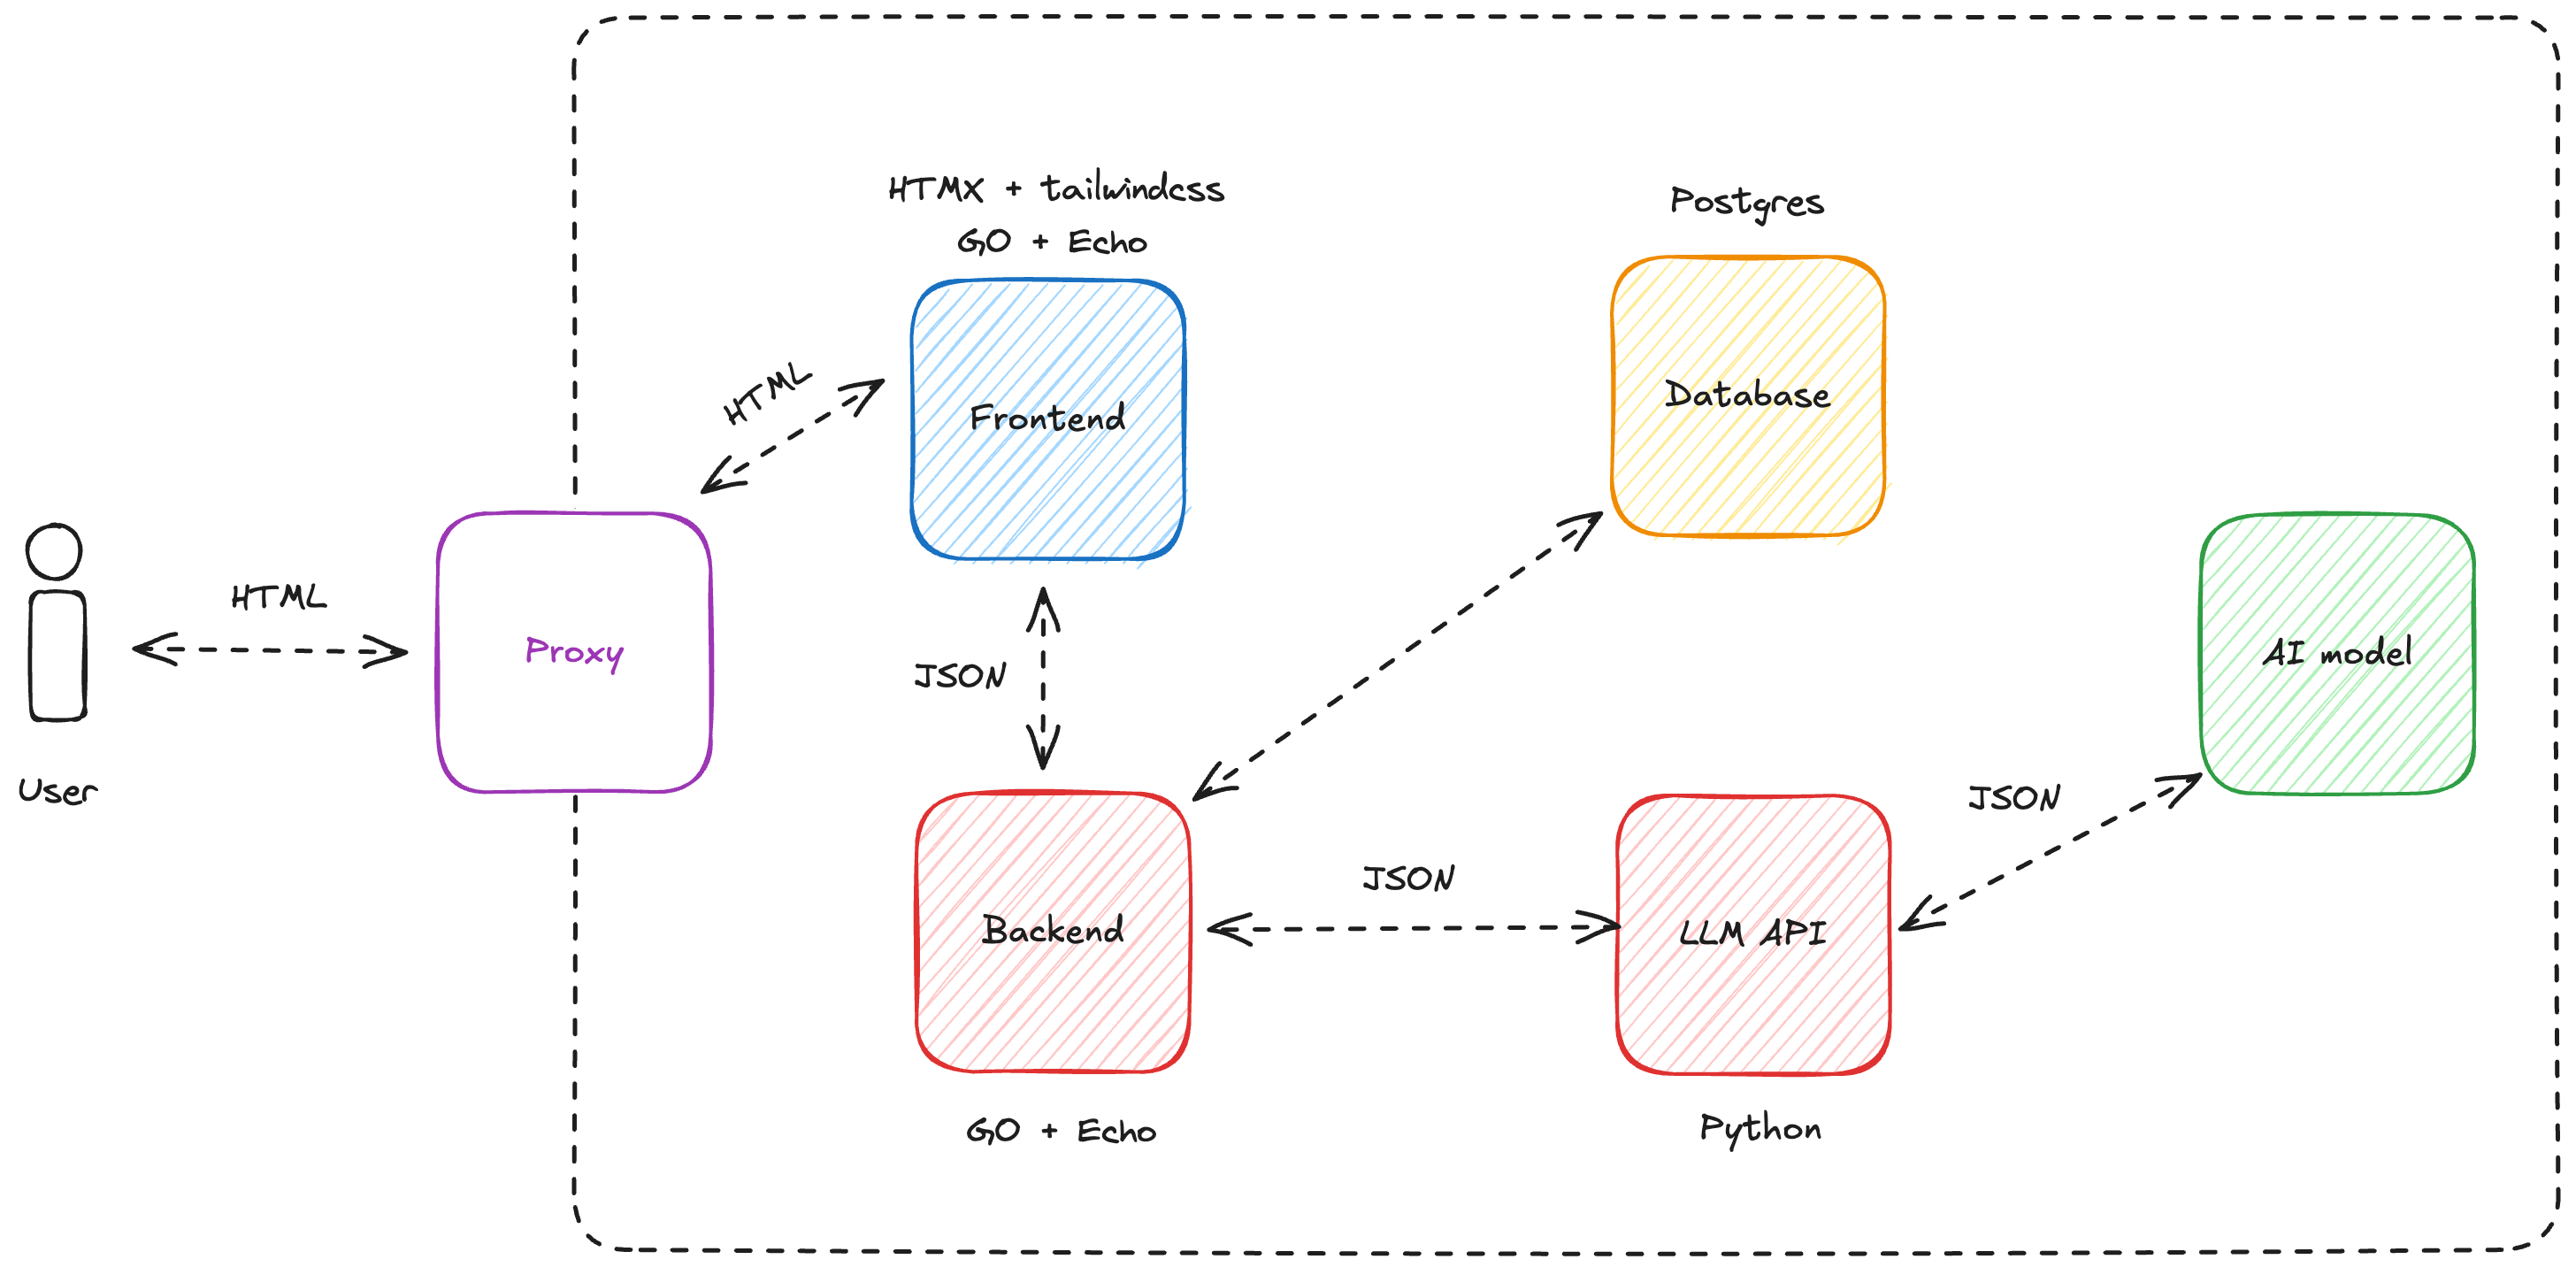
\includegraphics[width=0.8\textwidth, keepaspectratio]{figures/high-level-architecture.png}
    \caption{High-level system architecture}
    \label{fig:high-level-architecture}
\end{figure}

The frontend server is the part of the platform that users interact with directly. It's built as a server-rendered HTMX application using the Go programming language and the Echo framework. As the main entry point to the platform, it processes user inputs, communicates with the backend service, and provides content to users.

The backend is also written in Golang using the Echo framework. It is a regular REST application that communicates with HTTP requests. It brings together the different parts of the application and is responsible for the platform's business logic.

The database is Postgres, a popular, open-source relational database software. It stores all the data so the platform can work seamlessly. This component only communicates with the backend service.

The LLM API component is a unified interface for accessing the AI model. It is a small Python web application with a REST interface for more accessible communication. It contains prompts and question generation-related business logic. The component enables the platform to integrate different AI models or change between them on the fly.

The AI model component is a small application containing the question generator LLM. Máté Debreczeni fine-tuned the pre-trained llama-3-8B\footnote{https://huggingface.co/meta-llama/Meta-Llama-3-8B} model for the platform on a custom dataset he created from Wikipédia articles \footnote{https://en.wikipedia.org/wiki/Wikipedia:Vital_articles}. He aims to train a model that generates better-quality questions in the given format than the starter model.  

\subsection{Example component interaction}

Figure \ref{fig:component-interaction} shows an example interaction between the components through a question generation. This interaction is the primary interaction between the components and utilizes all of them.

\begin{figure}[!h]
    \centering
    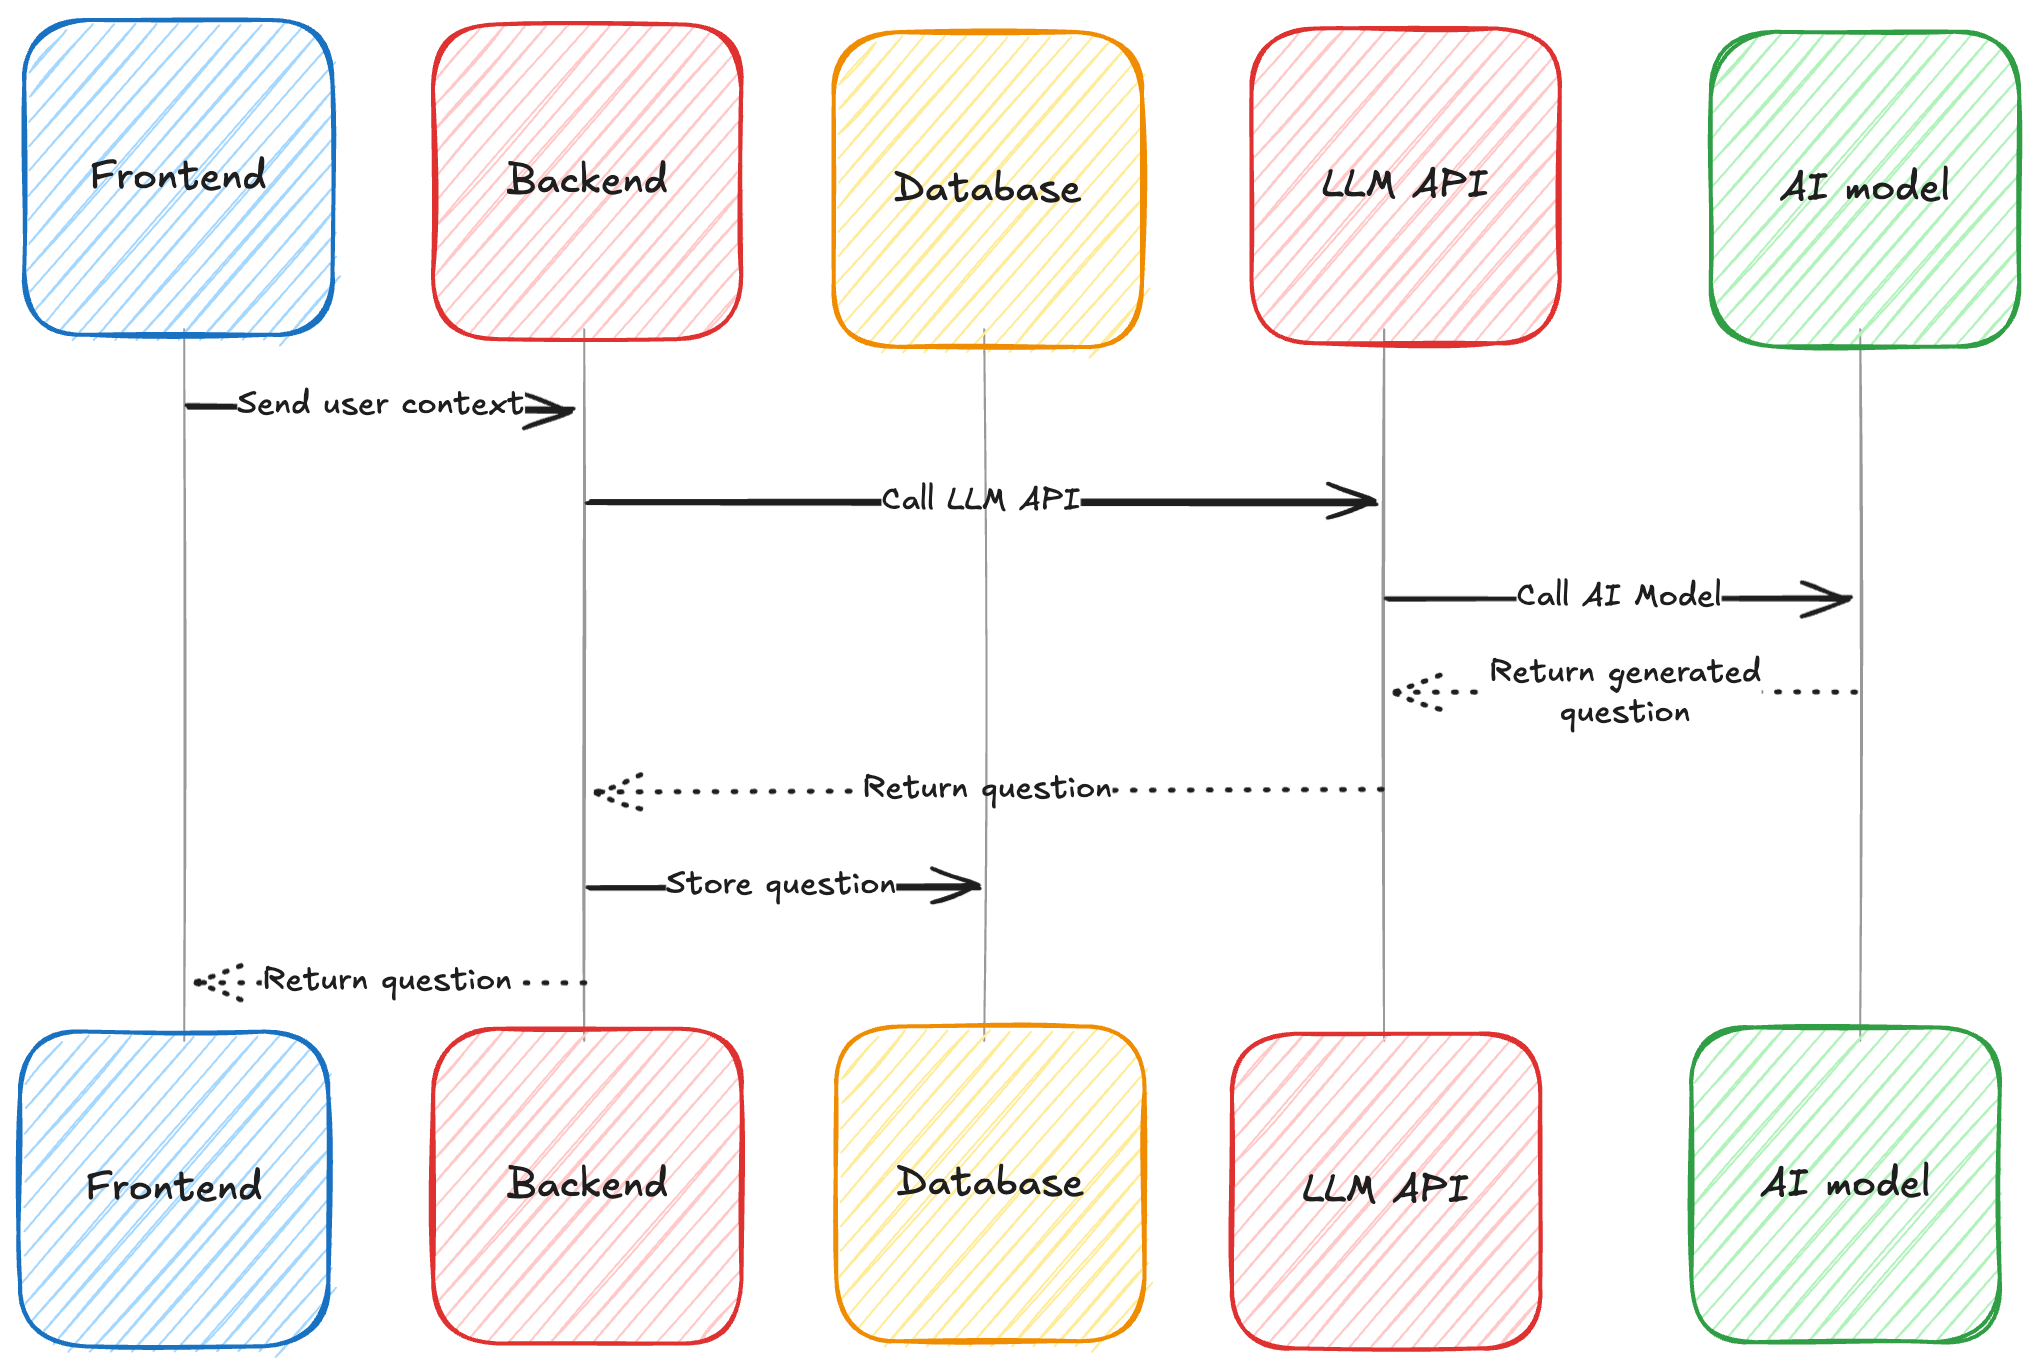
\includegraphics[width=0.8\textwidth, keepaspectratio]{figures/component-interaction.png}
    \caption{Component interaction: Question generation}
    \label{fig:component-interaction}
\end{figure}

Users submit their context to the frontend server, which validates the input and sets parameters like question type and quiz ID. The frontend calls the backend's proper endpoint with these parameters. The backend also validates the request and calls the LLM API to generate the question. The LLM API delegates the generation to the AI model through a request containing a pre-created prompt. This question is returned to the backend, where additional data is added and saved to the database. Finally, the backend returns the question to the frontend for display to the user.

\subsection{Deployment design}

Containerization is a crucial part of platform development and deployment. From the start, all the components were containerized with Docker for easier development and to ensure they worked on other machines. Máté worked on the AI model and the LLM API, and I worked on the other parts. Both of us used different operating systems, software, and tools. Without this method, we could not have worked together as efficiently as we did.

We created a Dockerfile for each service that describes how to build and run the respective application. We configured a docker-compose file to make them work together. We also considered building containers efficiently using the multi-layered containerizing approach. This idea was essential for the frontend and the backend due to the code generation, which has to be performed frequently.

\subsubsection{Development deployment}

Figure \ref{fig:dev-deployment} shows how we deployed locally the platform for development. It consists of two groups: the local environment and the external environment. The local environment has all of the components in the system architecture diagram; this is a complete system. In comparison, the external environment consists of only one service, an LLM from Google. It is the company's fastest Gemini model (gemini-1.5-flash). 

The LLMs, even these smaller ones, need a lot of resources. Thus, question generation usually takes over a minute on a personal computer. We sped up the development process using Gemini's API when developing and testing the services.

\begin{figure}[!h]
    \centering
    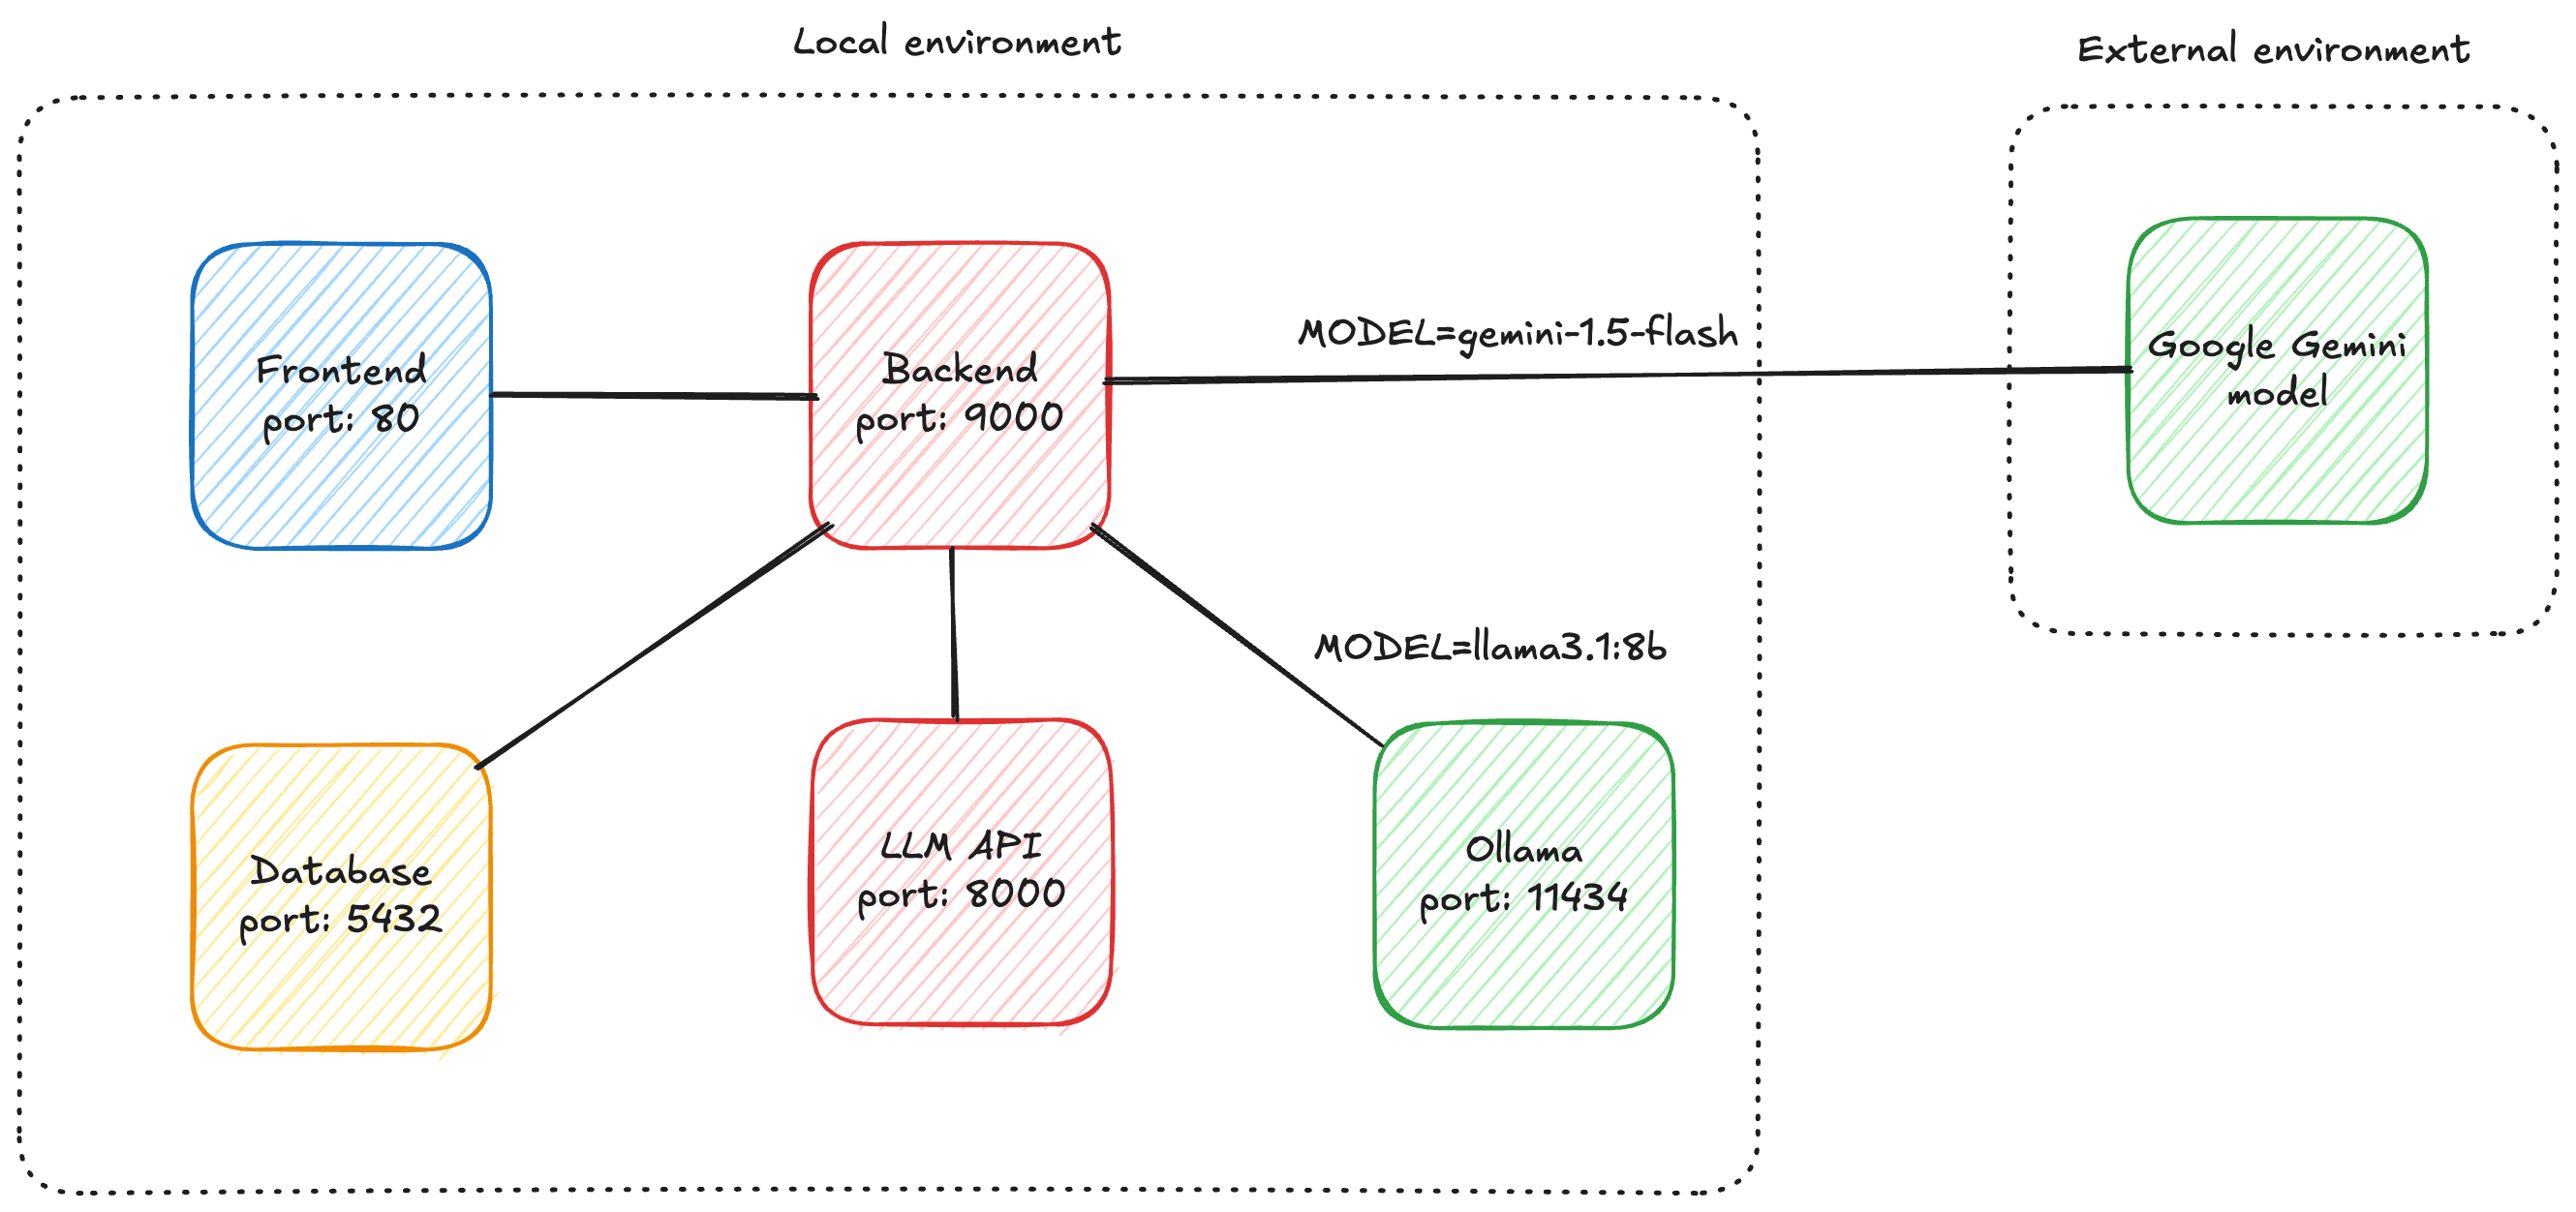
\includegraphics[width=0.8\textwidth, keepaspectratio]{figures/dev-deployment.png}
    \caption{Developer deployment}
    \label{fig:dev-deployment}
\end{figure}

\subsubsection{Production deployment}

We use a similar structure for production but without the Gemini model. We also split up the parts in this case into two, as Figure \ref{fig:production-deployment} shows. The regular services (frontend, backend, database, LLM API) are found on Máté's VPS (Virtual Private Server) in a Kubernetes\footnote{https://kubernetes.io/} cluster, while the AI model is deployed to an external provider. The VPS has no GPU; thus, we selected a provider specializing in running LLMs.

\begin{figure}[!h]
    \centering
    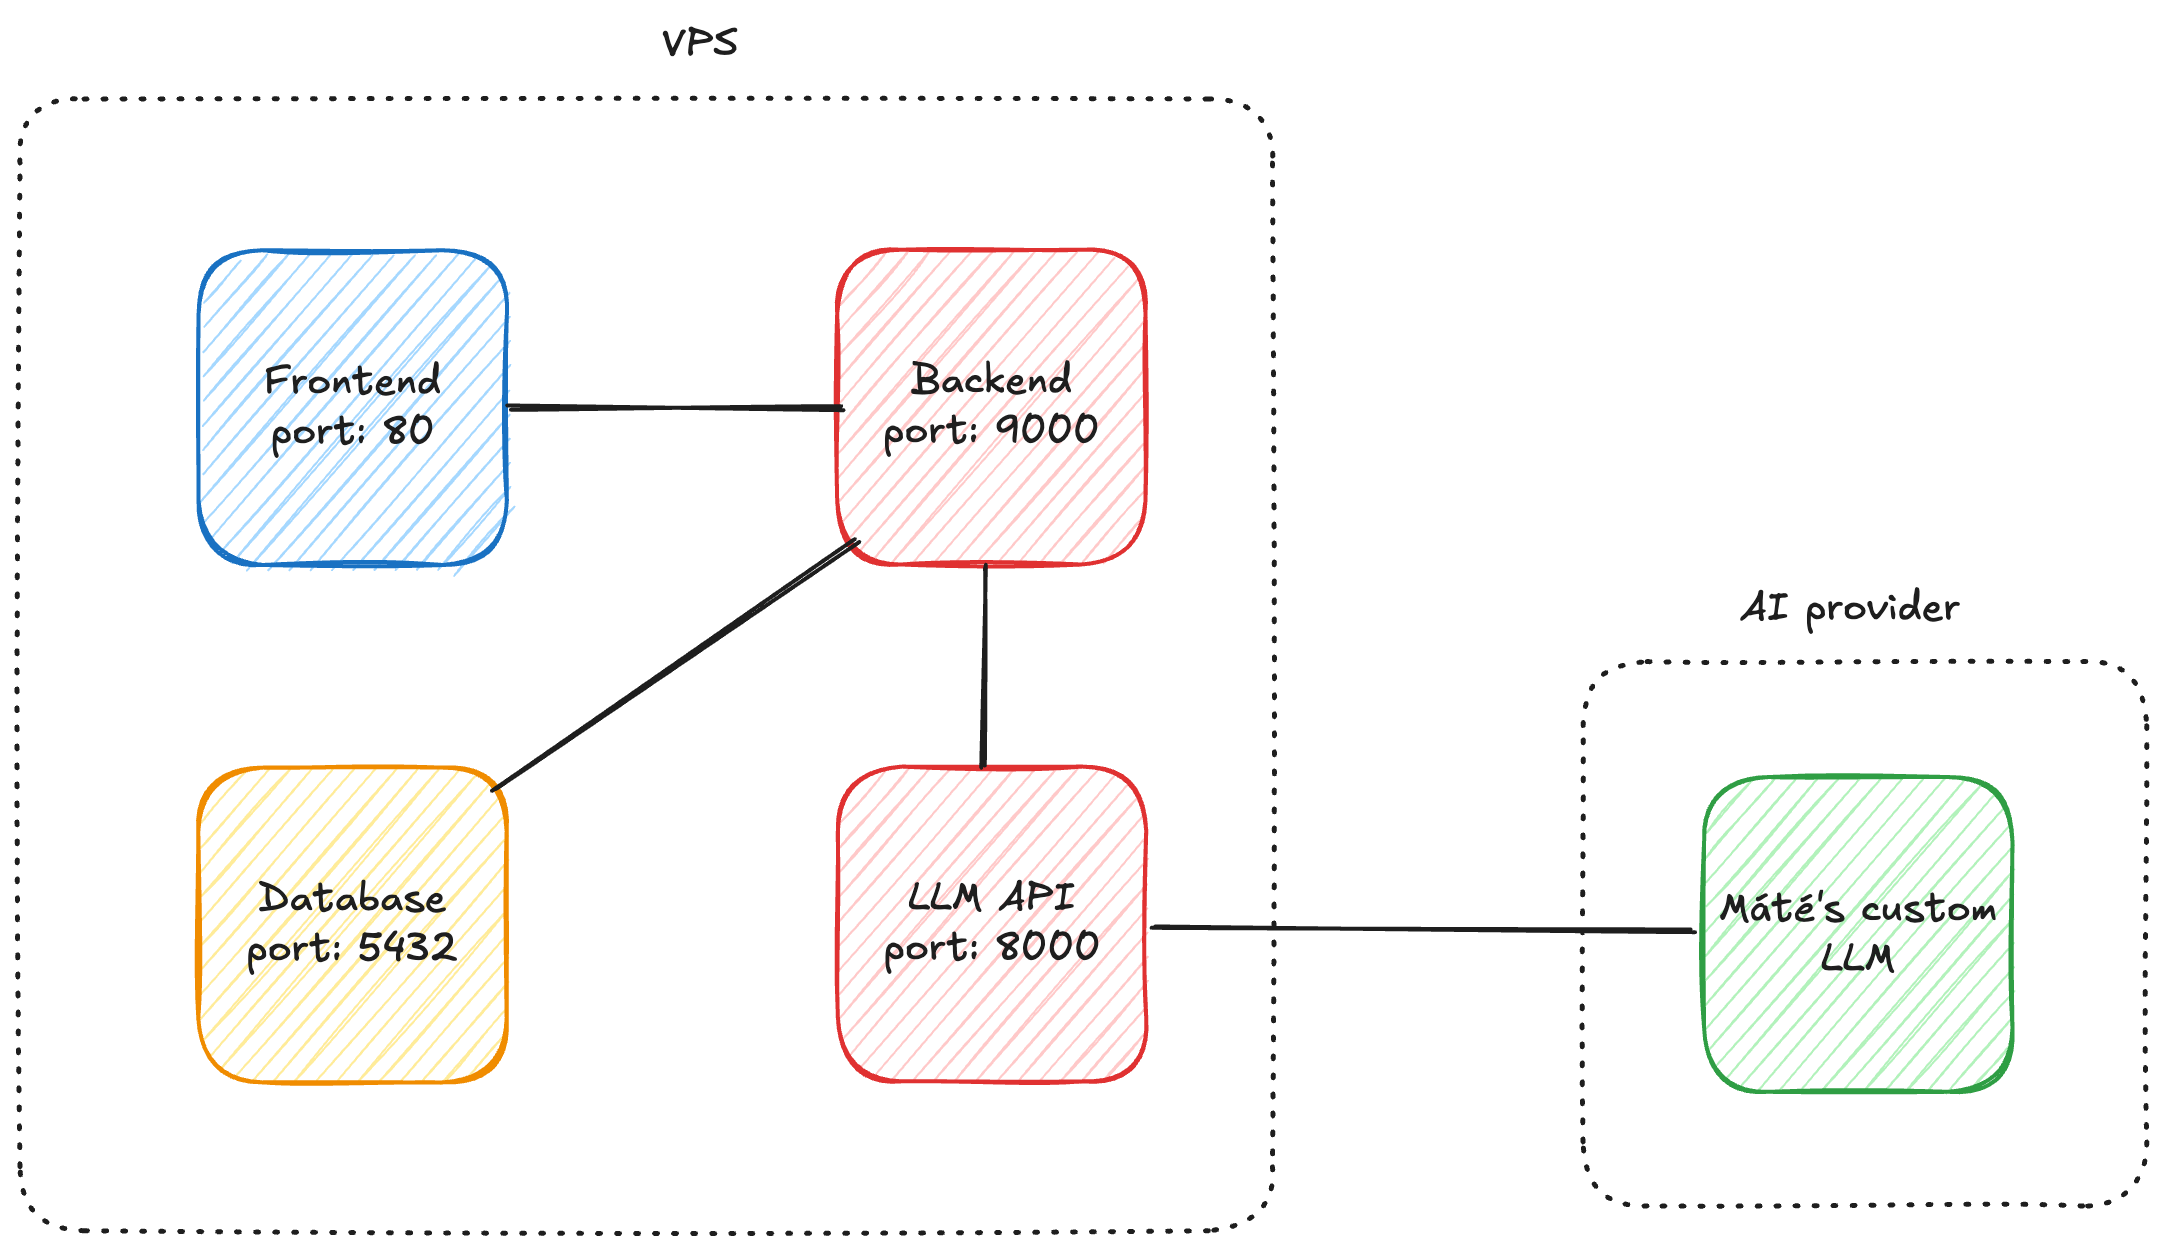
\includegraphics[width=0.8\textwidth, keepaspectratio]{figures/production-deployment.png}
    \caption{Production deployment}
    \label{fig:production-deployment}
\end{figure}

\section{Database Design}

Database design and software selection are critical parts of every web application; the same applies to the platform. Thus, we chose a relational database, Postgres, to store and serve the platform's data. I write about the database software selection and its rationale after introducing the data model from multiple aspects and the decisions behind them.

\subsection{Database software selection}

Postgres is one of the most popular Database Manager System (DBMS) software available today. It is free and open-source and offers a ready-to-use solution as a Docker container. We have worked with it for different projects through the years, and it has always been a good choice. So, its familiarity and reliability were the most important reasons for selecting it, besides its performance and wide adaption at database providers. 

Although it is a traditional database, it is extendable with third-party extensions. Its package manager is called trunk\footnote{https://pgt.dev/}, and it is effortless to install database packages by using it. We installed pgvector\footnote{https://github.com/pgvector/pgvector} for vector database features for the AI and another one called pgchron\footnote{https://github.com/citusdata/pg_cron} for scheduling session-related tasks.

\subsection{Entity-Relationship diagrams}

This section discusses the entities and their relationships in the application at this layer. I split it up into six smaller parts for easier understanding and overviewing.

\subsubsection{Users and sessions}

The database has two entities tightly connected to the user: User and Session. The User entity holds regular information about the user, like name, email, and hashed password, while the session stores the current user's session and its validity. When the user authenticates, a session is created and sent to the user's computer as a session cookie for later use. The session ID is used for authentication throughout the whole platform and has an expiration date when a pgchron task automatically deletes it. Figure \ref{fig:er-user-and-session} displays the entities and the relationship between them.

\begin{figure}[H]
    \centering
    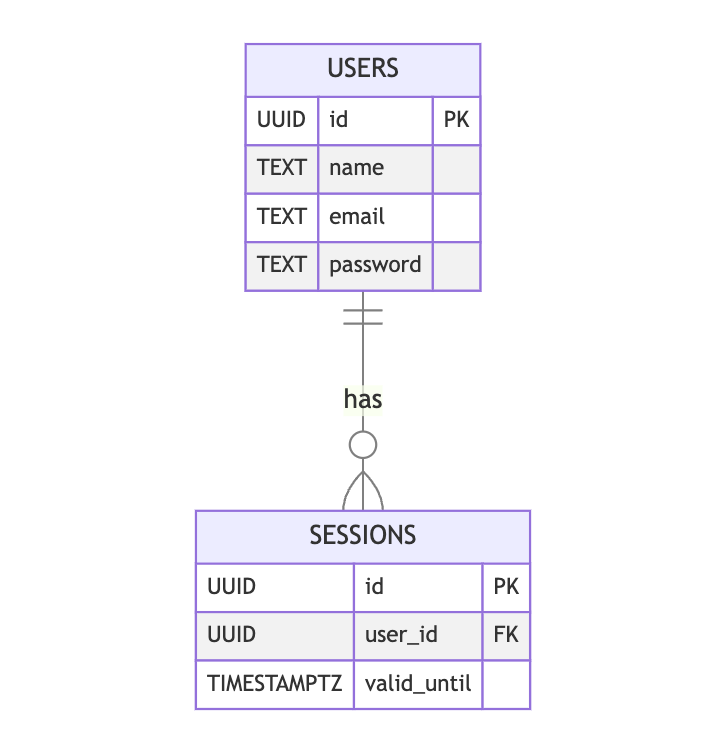
\includegraphics[width=0.8\textwidth, keepaspectratio]{figures/er-user-and-session.png}
    \caption{ER Diagram: User and Session}
    \label{fig:er-user-and-session}
\end{figure}

\subsubsection{Quizzes and questions}

The platform's core entities are the Quizzes and their questions. Each quiz has a name, description, and creator and is linked to different types of questions. There are three types of questions: SingleChoiceQuestion, a question with only one correct answer; MultipleChoiceQuestion, which can have multiple correct answers; and TrueOrFalseQuestion, aka a boolean question. Each type has its entity and table in the database. They are mostly the same; they all have a more extended text field describing the question and differ in the answer type.

The quizzes can be accessed through a QuizAccess entity, which links the user to a quiz with a role. By default, an instance with an owner role is generated automatically when a user creates a quiz. This abstraction allows controlling which quiz can be viewed or edited by whom. It also makes it available for future development as a platform for sharing private quizzes or creating public ones. Figure \ref{fig:er-quizzes} displays the quizzes, types of questions, and accesses in an ER diagram.

\begin{figure}[H]
    \centering
    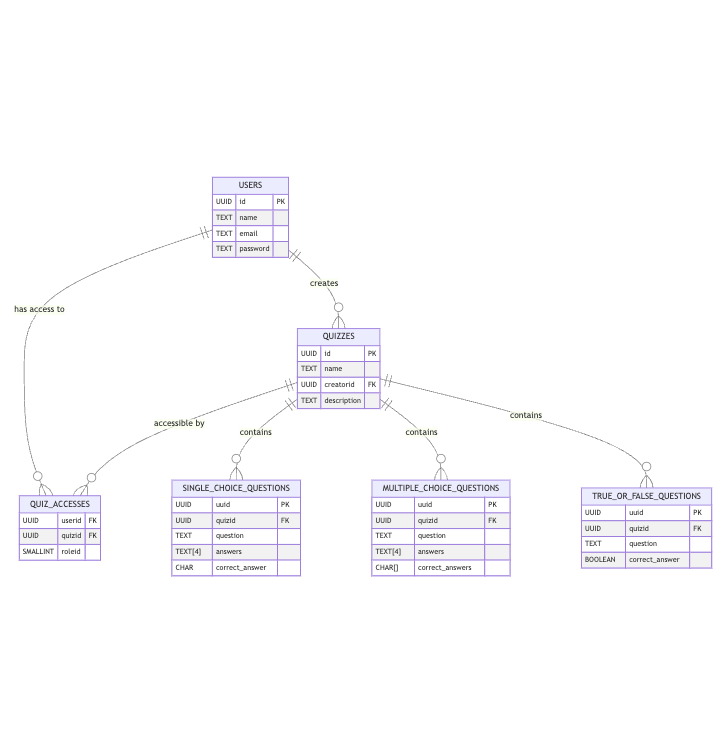
\includegraphics[width=0.8\textwidth, keepaspectratio]{figures/er-quizzes.png}
    \caption{ER Diagram for quizzes and questions}
    \label{fig:er-quizzes}
\end{figure}

\subsubsection{Quiz sessions}

Another essential entity category is related to answering questions. The central entity is the QuizSession, which holds the information together for quiz completion. It accounts for start and finish time and links to answers connected to questions. And it is also related to the quiz result if it is submitted. Some answer entities hold the information of the user's answer to the given question. Figure \ref{fig:er-quiz-session} shows these relations.

\begin{figure}[H]
    \centering
    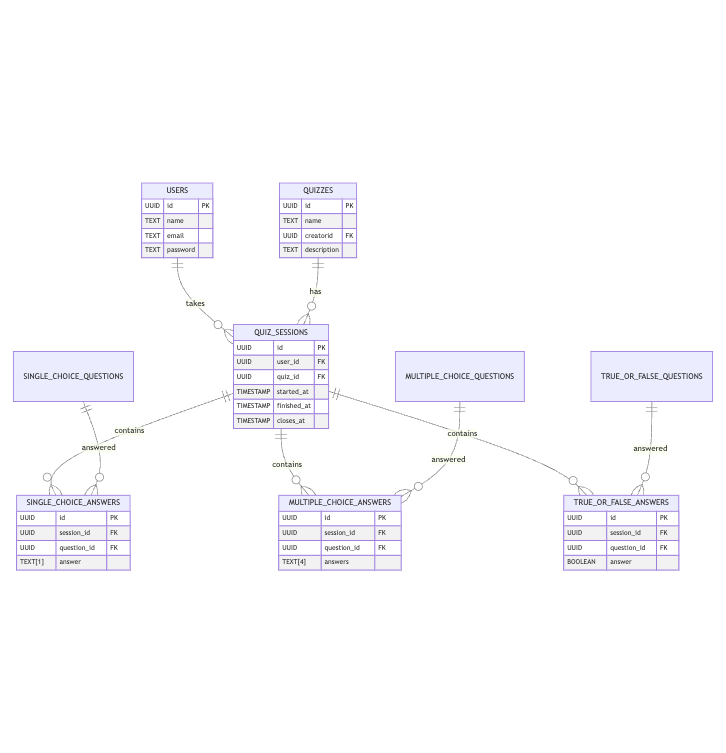
\includegraphics[width=0.8\textwidth, keepaspectratio]{figures/er-quiz-sessions.png}
    \caption{ER Diagram for quiz sessions}
    \label{fig:er-quiz-session}
\end{figure}

\subsubsection{Answers and quiz results}

In addition to the entities detailed before, there are more entities related to QuizSession, but now, it is for storing the scores for the answers and the results of the finished one. When a quiz is submitted and the session is finished, AnswerScore entities are created, which store the user's score for their given answers, and a question result record is also added with total scores. QuizResult is just a supporting entity for later extensibility capabilities; currently, it could have been merged into the QuizSession. 

\begin{figure}[H]
    \centering
    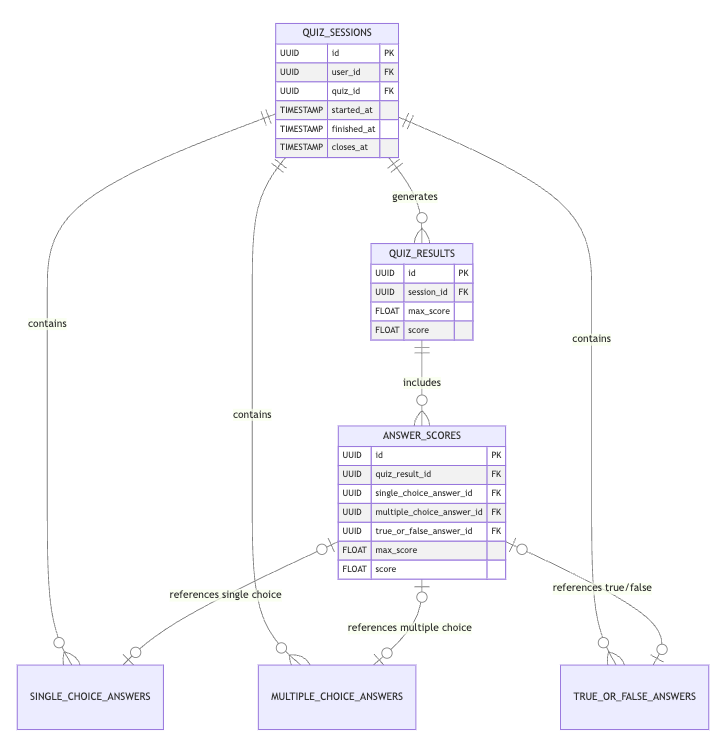
\includegraphics[width=0.8\textwidth, keepaspectratio]{figures/er-quiz-result.png}
    \caption{ER Diagram for answers and quiz results}
    \label{fig:er-quiz-result}
\end{figure}

Each AnswerScore has a max\_score and score field, which holds the maximum available and the obtained score. It establishes three distinct relationships corresponding to different question types. These relationships are structured with cardinality constraints, ensuring that a single AnswerScore can be linked to only one question at a time, maintaining a one-to-zero or one-to-one connection depending on the specific question type. Figure \ref{fig:er-quiz-result} shows all the entities and relations mentioned in these paragraphs.

\subsubsection{Learn list}

\begin{figure}[H]
    \centering
    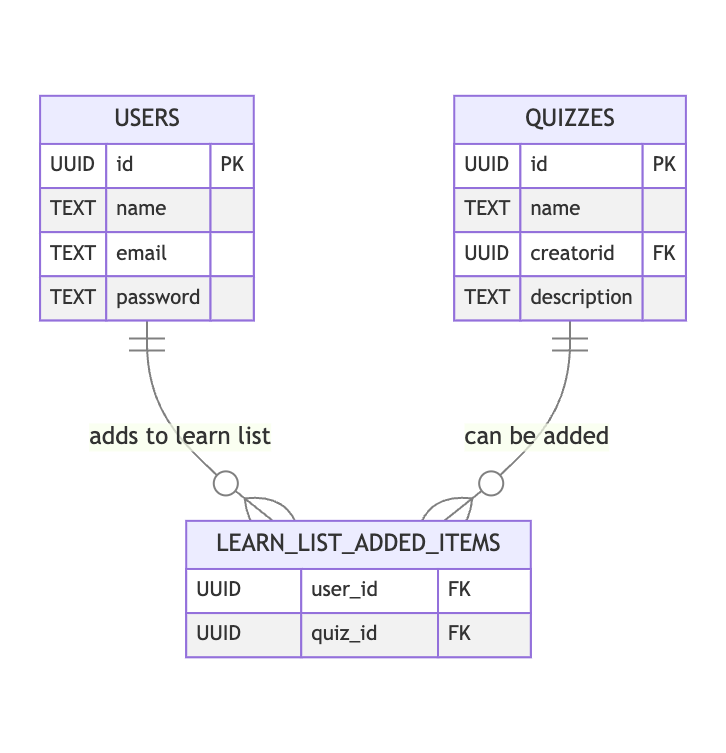
\includegraphics[width=0.8\textwidth, keepaspectratio]{figures/er-learn-list.png}
    \caption{ER Diagram for learn list}
    \label{fig:er-learn-list}
\end{figure}

\subsubsection{Review items}

\begin{figure}[H]
    \centering
    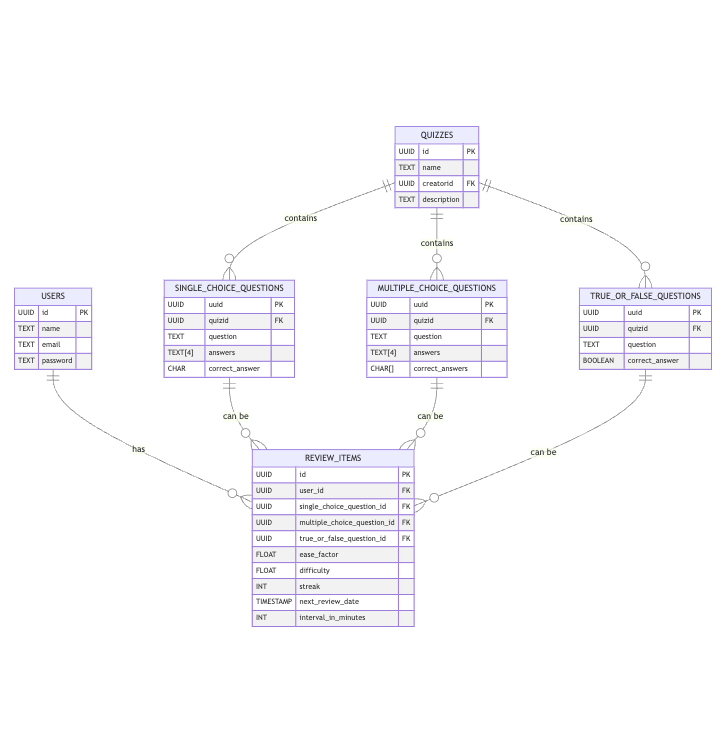
\includegraphics[width=0.8\textwidth, keepaspectratio]{figures/er-review-items.png}
    \caption{ER Diagram for review items}
    \label{fig:er-review items}
\end{figure}

\subsection{Database schema}

\subsection{Key tables and their relationships}

\subsubsection{Core tables}
    
\subsubsection{Supporting tables}
    
\subsection{Data modeling decisions}

\subsubsection{Indexing strategy}

\subsubsection{Data type selection}

\subsubsection{Constrains and integrity rules}

\section{Frontend Design}

\subsection{User Interface (UI) design principles}

\subsubsection{Chosen design metolodogy}

\subsubsection{User experience (UX) goals}

\subsubsection{Design system planning}

\subsection{Architecture Planning}

\subsubsection{Selected frontend architecture pattern and rationale}
        
I adopted a server-side-driven architecture using HTMX and Go for the application. It is a Multi-Page Architecture (MPA) at the core but leverages the framework's SPA-like capabilities. The architectural pattern consists of server-side HTML generation, HTMX enhancement, and the component structure.

The server generates the pages dynamically using the templating engine called templ. The dynamic content is served through partial HTML updates with HTMX requests. This way, the server controls the UI state instead of the client. The approach has several benefits: it decreases the initial site load and simplifies state management because the client receives the complete page containing the client state.

The HTMX library provides the interactions with its AJAX request boosting feature. Applications using the framework can act like single-page applications because the in-place content updates could replace full-page reloads. The approach offers progressive enhancement by not requiring rewriting everything initially and reduces writing additional JavaScript even to zero lines.

The UI is organized into reusable components. They are written in Go using templ.

\subsubsection{Component hierarchy planning}

\subsubsection{}

\section{Backend Design}

\section{AI integration Design}